%
% project plan
% @author Tobias Weber <tweber@ill.fr>
% @date jan-2021
% @license see 'LICENSE' file
%

\chapter*{Abstract}
\addcontentsline{toc}{chapter}{Abstract}

The triple-axis spectrometer (TAS) \cite{Shirane2002} was invented by B. Brockhouse in the 1950s and 
is among the foremost measurement methods in the field of inelastic neutron scattering. 
It enables the probing of vibrational (phonon) or magnetic (magnon) excitations in single crystals and allows 
mappings of their dispersion relations, i.e. their energy-momentum relation, $E\left( \bm{Q} \right)$.

The three axes of a TAS are offset by relative angles to one another, and comprise 
(i) the reactor-monochromator-sample axis, where a specific neutron energy is picked out of the polychromatic 
beam coming from the reactor's moderator; 
(ii) the monochromator-sample-analyser axis, whose angle selects a specific momentum transfer, $\bm{Q}$, 
from the neutron to the sample; and 
(iii) the sample-analyser-detector axis, which selects the energy transfer, $E$.

During the usual operation of a TAS, the user selects $\left( \bm{Q}, E \right)$ coordinates in the reciprocal (dual)
crystal space of the sample to be measured. While the vector space of crystal coordinates 
is in general non-Euclidean, crystal coordinates have a one-to-one correspondence with the axis angles 
of the TAS. The correspondence can be calculated by the so-called ``$UB$ matrix formalism'' \cite{Lumsden2005}. 
Here, $B$ is the transformation matrix from crystal to lab coordinates and $U$ is a rotation to a specific 
crystal plane. From that, the TAS angles can be derived using Bragg's law.

Due to angular constraints by cables and tubes, as well as spatial constraints from the crammed instrument space, 
not every $\left( \bm{Q}, E \right)$ coordinate point is accessible, and a careful mapping of each point is
usually required beforehand to avoid collisions of the instrument with walls, collisions with itself or movements
which could pull out fragile cables.

The goal of the proposed project is the development and implementation of a path-finding algorithm for 
neutron triple-axis spectrometers. Given a user-selected target coordinate in reciprocal crystal space, 
the algorithm will be able to navigate the instrument in its constrained angular space. The problem is similar to 
moving a robot arm around obstacles, with the addition of having the start and target coordinates in a 
coordinate system with a different metric.

%\begin{figure}[ht]
%	\begin{centering}
%	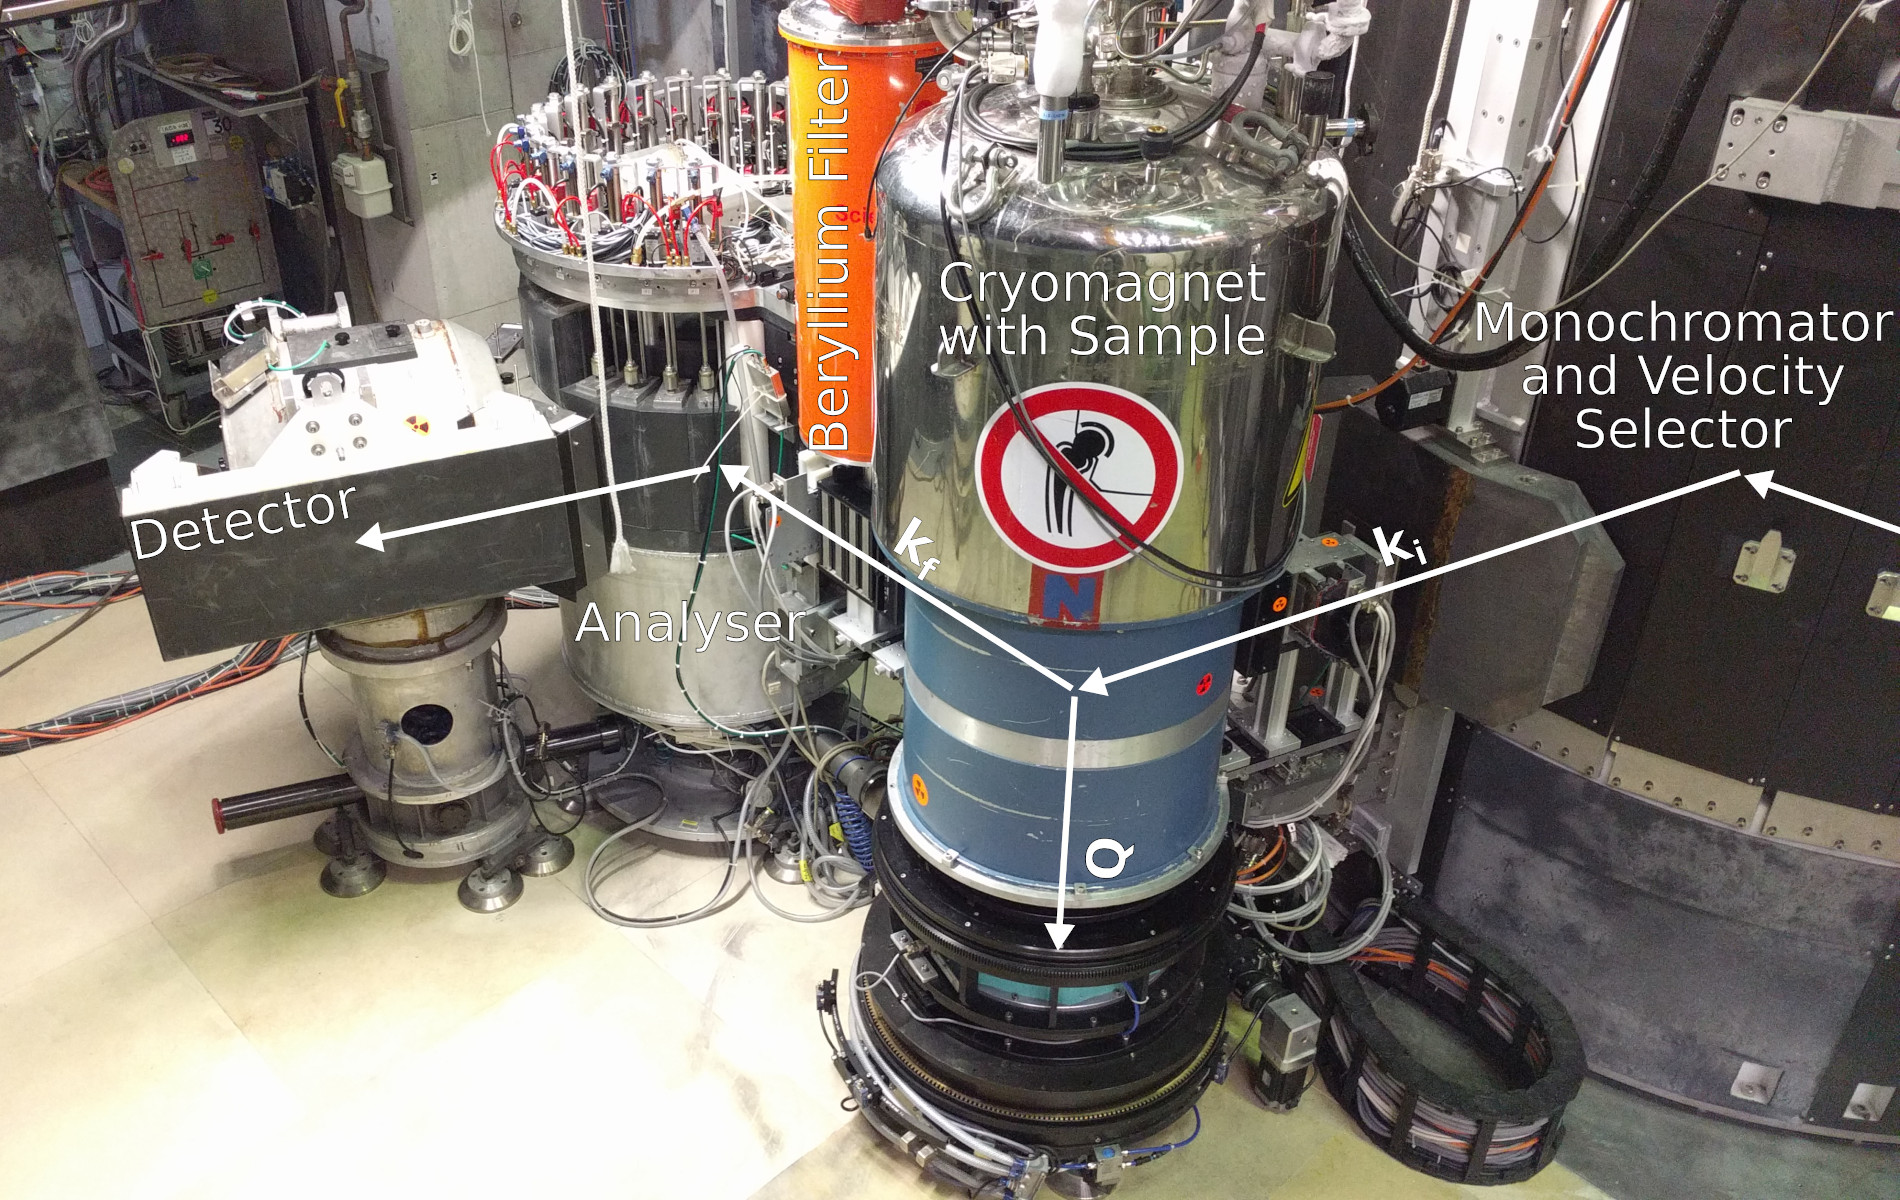
\includegraphics[width=0.66\textwidth]{figures/thales.jpg}
%	\end{centering}
%	\caption{The picture shows the triple-axis spectrometer \textit{ThALES} \cite{thales} at the ILL.}
%	\label{fig:tas}
%\end{figure}
